% ---------------------------------
% Describe document characteristics
% ---------------------------------

\documentclass[12pt]{article}

% Classic packages

\usepackage{fullpage} %full page typesetting -- defaults to 1 inch margins
\usepackage{setspace} %allows for non-singlespacing
\usepackage{latexsym} %extra symbols
\usepackage{rotating} %rotation for figures
\usepackage{longtable} %tables that fill more than a single page
\usepackage{natbib} %better bibliographies
\usepackage{authblk} %author and affiliation in opening

% Paper Abstract

\usepackage{abstract}
\renewcommand{\abstractname}{}    % abstractname replaced with NULL
\renewcommand{\absnamepos}{empty} % removes the block where abstract would
								  %   have been placed, originally 'center'

% Shortcut Commands

\newcommand\e{\emph} %Italics
\newcommand\tb{\textbf} %Bold
\newcommand\un{\underline} %Underline
\newcommand\txt{\texttt} %Code
\newcommand\tsc{\textsc} %Small Caps

% Change Section Header looks

\usepackage[rm, small, sc]{titlesec} % titles are non-bold, small, caps
\titleformat*{\subsection}{\itshape} % subsection titles are italic
\titleformat*{\paragraph}{\itshape}  % paragraph titles are italic

% Links
\usepackage{hyperref} %hypertext links in the document
\hypersetup{
	colorlinks=true,
	linkcolor=blue,
	filecolor=magenta,      
	urlcolor=cyan,
	citecolor=black
}

% Graphics
\usepackage{graphicx} %graphics capabilities
\graphicspath{ {Images/} } % Use the Images folder to hold images

% Tables
\usepackage{tabulary}
\usepackage{booktabs}
\usepackage{caption}
\usepackage{float}

% Math
\usepackage{amsmath} % math functions
\usepackage{amssymb} % math symbols

% Code
\usepackage{listings}
\lstset{
	numbers=left, 
	numberstyle=\small, 
	numbersep=8pt, 
	frame = single, 
	language=Pascal, 
	framexleftmargin=15pt}
% No numbers
%\lstset{
%	basicstyle=\ttfamily,
%	columns=fullflexible,
%	frame=single,
%	breaklines=true
%}

% Multiple Colmns
\usepackage{multicol}

% ---------------------------------
% Document Parameters
% ---------------------------------

% Spacing
\doublespacing

% Name and Title
\title{\tb{Paper Template}}
\author{Jennifer Lin}
\affil{Northwestern University}
\date{} %For No Date appearance
%\date{\today} %For Date to Today

% ---------------------------------
% Writing
% ---------------------------------

\begin{document}

% Title creation
\begin{singlespace}
	\maketitle
\end{singlespace}

% Insert Abstract Here
\begin{abstract}
	Sample Abstract
\end{abstract}

\begin{singlespace}
	\tableofcontents
\end{singlespace}

% Horizontal line after TOC
\noindent\rule[0.5ex]{\linewidth}{0.5pt}

% Begin Paper Construction

\section{Introduction}

Begin Writing paper here

\subsection{A Subsection}

I am citing a paper here \cite{graham2009liberals}

\section{Tables and Graphics}

Here is a table using the \txt{booktabs} package

\begin{singlespace}
	

\begin{table}[H]
	\centering
	\caption{\e{Caption for the Table}}
	\label{table}
	\begin{tabular}{lcccc}
		\toprule
		&\multicolumn{2}{c}{Instances}&&\\
		\cmidrule{2-3}
		Foundation& Democrat &Republican &\e{t}& Effect Size (\e{d})\\
		\midrule
		Harm&9.03& 10.7&-0.867&-0.144\\
		Fairness&2.04&2.84&-1.260&-0.222\\
		Ingroup&3.34&5.34&-2.487*&-0.431\\
		Authority&3.20&8.97&-5.053***&-1.007\\
		Purity&1.88&4.06&-4.347***&-0.714\\
		\bottomrule
	\end{tabular} \\
	\begin{minipage}{10cm}
		~~\\
		\e{Notes:} 
		(*)\e{p} = .1, *\e{p} = .05, **\e{p} = .01, ***\e{p} $\leq$ .001
	\end{minipage}
\end{table}

\end{singlespace}

\noindent Here is a Figure

\begin{figure} [H]   
	\centering
	{	 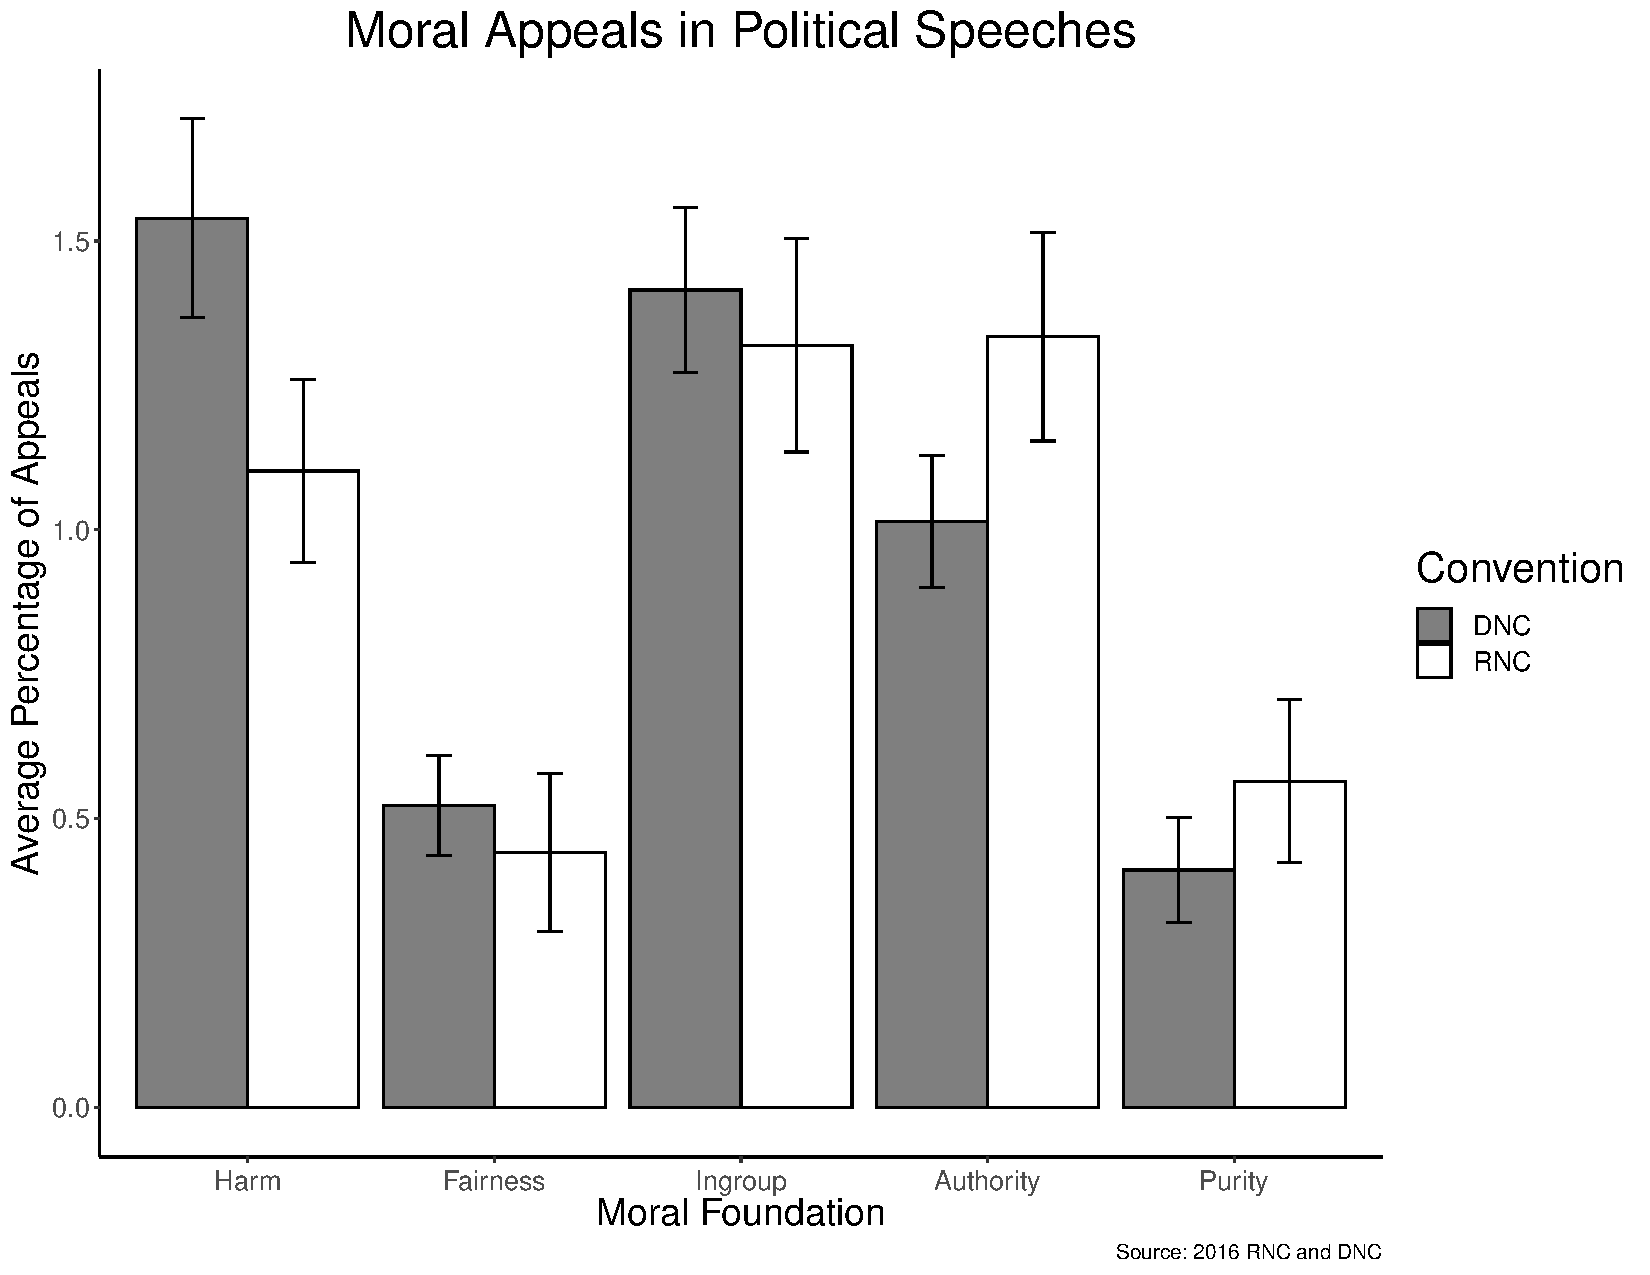
\includegraphics[width=.7\textwidth]{graph}}
	\caption{Caption for the graph}\label{figure}
\end{figure}

\subsection{Math Equations}

Here is a math equation in two ways

\begin{equation}
E=mc^2
\end{equation}

\[E=mc^2\]

\section{Insert Code}

\begin{singlespace}
\begin{lstlisting}[language=Python]
import numpy as np

def incmatrix(genl1,genl2):
	m = len(genl1)
	n = len(genl2)
	M = None #to become the incidence matrix
	VT = np.zeros((n*m,1), int)  #dummy variable

#compute the bitwise xor matrix
	M1 = bitxormatrix(genl1)
	M2 = np.triu(bitxormatrix(genl2),1) 

for i in range(m-1):
for j in range(i+1, m):
	[r,c] = np.where(M2 == M1[i,j])
for k in range(len(r)):
	VT[(i)*n + r[k]] = 1;
	VT[(i)*n + c[k]] = 1;
	VT[(j)*n + r[k]] = 1;
	VT[(j)*n + c[k]] = 1;

if M is None:
	M = np.copy(VT)
else:
	M = np.concatenate((M, VT), 1)

VT = np.zeros((n*m,1), int)

return M
\end{lstlisting}
\end{singlespace}

\section{Multiple Columns text}

\begin{multicols}{2}
	thing 1 \\
	thing 2
\end{multicols}

% Bibliography Section

\begin{singlespace}
	%\def\bibfont{\footnotesize}
	\bibliographystyle{chicago}
	\bibliography{References}
\end{singlespace}

\end{document}




